%\documentclass[handout]{ximera}
\documentclass{ximera}


\graphicspath{
  {./}
  {graphics/}
  {../graphics/}
}

\usepackage{chngcntr}

\let\question\relax
\let\endquestion\relax




\newtheoremstyle{SlantTheorem}{\topsep}{\fill}%%% space between body and thm
%\newtheoremstyle{SlantTheorem}{\topsep}{\topsep}%%% space between body and thm
 {\slshape}                      %%% Thm body font
 {}                              %%% Indent amount (empty = no indent)
 {\bfseries\sffamily}            %%% Thm head font
 {}                              %%% Punctuation after thm head
 {3ex}                           %%% Space after thm head
 {\thmname{#1}\thmnumber{ #2}\thmnote{ \bfseries(#3)}}%%% Thm head spec
\theoremstyle{SlantTheorem}
\newtheorem{question}{Question}
\counterwithin*{question}{section}



\let\instructorNotes\relax
\let\endinstructorNotes\relax
%%% instructorNotes environment
\ifhandout
\newenvironment{instructorNotes}[1][false]%
{%
\def\givenatend{\boolean{#1}}\ifthenelse{\boolean{#1}}{\begin{trivlist}\item}{\setbox0\vbox\bgroup}{}
}
{%
\ifthenelse{\givenatend}{\end{trivlist}}{\egroup}{}
}
\else
\newenvironment{instructorNotes}[1][false]%
{%
  \ifthenelse{\boolean{#1}}{\begin{trivlist}\item[\hskip \labelsep\bfseries {\Large Instructor Notes: \\} \hspace{\textwidth} ]}
{\begin{trivlist}\item[\hskip \labelsep\bfseries {\Large Instructor Notes: \\} \hspace{\textwidth} ]}
{}
}
{\end{trivlist}}
\fi


%% Suggested Timing
\newcommand{\timing}[1]{{\bf Suggested Timing: \hspace{2ex}} #1}

\title{Geometry and Multiplying Complex Numbers}
\author{Bart Snapp and Brad Findell}

\outcome{Learning outcome goes here.}

\begin{document}
\begin{abstract}
Abstract goes here.  
\end{abstract}
\maketitle

\label{A:complexMultiplication}

Now we'll investigate the geometry of multiplying complex
numbers. In each case, specify the transformation.  For example, if you see a rotation, specify the angle and the center of rotation.  

Louie Llama\index{Louie Llama} is here to help us out:
\begin{image}
\begin{tabular}{ccc}
\includegraphics[scale=.5]{llama.pdf} & 
\qquad $\leftrightsquigarrow$\qquad & 
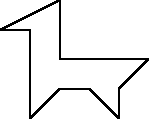
\includegraphics{llamaPlot.pdf}\\
Louie Llama & & how we'll draw him
\end{tabular}
\end{image}

\begin{problem} 
Here's Louie Llama hanging out near the point $0$ in the complex
plane. Multiply him by $2$. Make a table and show in the plane below what happens.  What transformation do you see?  
\begin{image}
\includegraphics{complexMult.pdf}
\end{image}
\end{problem}

\begin{problem} 
Now multiply him by $i$. Make a table and show in the plane below what happens.  What transformation do you see?  
\begin{image}
\includegraphics{complexPlane.pdf}
\end{image}
\end{problem}

\vfill

\begin{problem} 
Now multiply Louie Llama by $1+i$. Make a table and show in the plane
below what happens.  What transformation do you see?  
\begin{image}
\includegraphics{complexPlane.pdf}
\end{image}
\end{problem}

\vfill


\begin{problem} 
%  Used to mutliply by $\frac{1}{2}+\frac{\sqrt{3}}{2}i$.
Now multiply Louie Llama by $1 - 2i$. Make a
table and show in the plane below what happens.  What transformation do you see?  
\begin{image}
\includegraphics{complexPlane.pdf}
\end{image}
\end{problem}


\begin{problem}
Make a table to summarize your results from the previous problems.  
Then describe what happens geometrically when we ``multiply''  by a complex
number. 
\end{problem}

\end{document}
